\documentclass[11pt]{article}

\usepackage[margin=1in]{geometry}
\usepackage[T1]{fontenc}
\usepackage[utf8]{inputenc}
\usepackage{lmodern}
\usepackage{amsmath}
\usepackage{amssymb}
\usepackage{booktabs}
\usepackage{array}
\usepackage{graphicx}
\usepackage{hyperref}
\usepackage{multirow}
\usepackage{pgfplots}
\usepackage{siunitx}
\usepackage{xcolor}

\pgfplotsset{compat=1.18}
\sisetup{round-mode=places,round-precision=3}

\title{Which Neural Networks Waste the Most Energy on Apple Silicon?\\
\large CPU-Only Inference Measurements with Supplemental Synthetic Trial Modeling}
\author{Aryan Shah\\
Texas Academy of Mathematics and Science\\
University of North Texas, USA\\
\texttt{aryanshah.2431@gmail.com}}
\date{}

\begin{document}
\maketitle

\begin{abstract}
This paper studies inference energy for five neural network architectures on a
single hardware platform: Apple Silicon under CPU-only PyTorch execution.
Rather than making broad cross-device claims, the paper focuses on a controlled
measurement setting in which MobileNetV3-Small, MobileNetV2, ResNet-18,
Tiny-ViT-5M, and EfficientNet-B0 are evaluated using the same runtime, input
shape, and measurement procedure. The central result is that architecture-level
complexity proxies such as FLOPs and parameter count do not fully explain
measured energy use on this platform, while latency tracks energy closely. To
strengthen the engineering evidence, this release also includes a separate
17-architecture local CPU latency sweep with 30 measured trials per architecture,
exact machine metadata, parameter counts, model size, MACs, FLOPs, and proxy
EDP columns. To support repeated-trial analysis of the original energy table,
the paper adds a strictly Apple-Silicon-only synthetic trial model based on a
residualized conditional WGAN-GP. Under the paper-aligned evaluation protocol,
the synthetic model reproduces the measured energy ranking exactly, matches the
grounded energy and latency distributions, and preserves derived power after
calibration. The synthetic component is used only as supplemental support for
the measured Apple-Silicon study, not as a replacement for direct hardware
measurements.
\end{abstract}

\section{Introduction}
Energy efficiency is a practical deployment constraint even when inference is
restricted to a single well-controlled hardware platform. On Apple Silicon,
models with similar theoretical complexity can still behave differently because
measured energy depends not only on FLOPs and parameter count, but also on
runtime behavior, scheduling, and memory interaction
\cite{horowitz2014,mittal2019,hardwareaware2019}. For that reason, the most
defensible version of this study is a narrow one: a direct comparison of model
architectures under the same Apple-Silicon CPU-only inference setup.

This paper therefore focuses on a single-device benchmark. Five architectures
were measured under the same PyTorch runtime and the same input shape on Apple
Silicon, producing a clean ranking by energy per inference. The paper asks two
main questions: which architecture is most energy-efficient in this measured
setting, and how well do common complexity proxies explain the measured result?

The synthetic component plays only a supporting role. The measured benchmark
reports mean energy, power, and latency, but it does not publish model-level
trial spreads. To support repeated-trial style analysis without expanding the
scope of the paper, a paper-aligned conditional GAN is used only within the
same Apple-Silicon setting. Its purpose is not to generalize across devices,
but to provide supplemental trial-level variation anchored to the measured
means.

\section{Related Work}
Research on efficient neural network deployment spans three relevant threads.
The first focuses on architecture design, including MobileNet, MobileNetV2,
MobileNetV3, and EfficientNet, which reduce computation through depthwise
separable convolutions, inverted residuals, and compound scaling
\cite{mobilenet2017,mobilenetv22018,mobilenetv32019,efficientnet2019}. A second
thread studies systems-level energy behavior on real hardware, emphasizing that
data movement, memory access, and execution backends often dominate the cost
captured by abstract FLOP counts \cite{horowitz2014,mittal2019,eyeriss2017}.
The third thread concerns synthetic or predictive modeling of hardware behavior,
where statistical or machine learning models are used when full measurement
campaigns are impractical.

This paper sits between the first two threads. The primary evidence remains a
measurement study on Apple Silicon, while the synthetic extension is used only
to model repeated-trial behavior under the same device and runtime scope.

\section{Methodology}
\subsection{Measured Inference Benchmark}
All original benchmark runs used CPU-only inference in PyTorch with a fixed
input tensor of size $1 \times 3 \times 224 \times 224$. Each model was
executed with warm-up iterations followed by repeated timed inference runs.
Inference was performed locally on Apple Silicon with background activity
minimized and \texttt{powermetrics} used for power sampling.

\begin{table}[ht]
\centering
\caption{Hardware and software platform used for the measured benchmark.}
\begin{tabular}{ll}
\toprule
Component & Specification \\
\midrule
Device & Apple MacBook Pro (Apple Silicon) \\
Execution mode & CPU-only inference \\
Runtime & PyTorch 2.10 \\
Operating system & macOS 26.2 \\
Memory & 8 GB RAM \\
Power measurement & \texttt{powermetrics} (\texttt{cpu powersampler}, 1 Hz) \\
\bottomrule
\end{tabular}
\end{table}

\subsection{Models Evaluated}
The benchmark covers five architectures chosen to span depthwise CNNs, a
baseline CNN, and a lightweight transformer-style model.

\begin{table}[ht]
\centering
\caption{Architectures evaluated in the Apple-Silicon benchmark.}
\begin{tabular}{l l S[table-format=2.2] S[table-format=1.2]}
\toprule
Model & Architecture type & {Params (M)} & {FLOPs (G)} \\
\midrule
MobileNetV3-Small & CNN (depthwise) & 2.54 & 0.22 \\
MobileNetV2 & CNN (depthwise) & 3.50 & 0.30 \\
ResNet-18 & CNN (baseline) & 11.69 & 1.82 \\
Tiny-ViT-5M & Transformer-based & 12.08 & 1.30 \\
EfficientNet-B0 & CNN (scaled) & 5.29 & 0.39 \\
\bottomrule
\end{tabular}
\end{table}

\subsection{Expanded Local Architecture Sweep}
In addition to the five directly energy-measured models, the repository now
contains a broader local CPU latency sweep over 17 self-contained PyTorch
architecture variants. This sweep was added to make the architectural comparison
less dependent on a five-row table and to report real repeated-trial variation.
Each architecture was run with input shape $1 \times 3 \times 224 \times 224$,
10 warm-up iterations, and 30 measured CPU-only float32 inference trials. The
benchmark script records the exact environment in
\texttt{measurement\_environment.json}; for the run reported here, the machine
was a MacBook Pro with an Apple M4 Pro, 24 GB RAM, macOS 26.2, Python 3.9.6,
and PyTorch 2.8.0, with \texttt{torch.set\_num\_threads(1)}.

This expanded sweep directly measures latency, not energy. The accompanying
\texttt{paper\_baseline\_comparison.csv} file includes parameters, model size,
MACs, FLOPs, latency statistics, throughput, and a clearly labeled constant-power
energy-delay proxy. The proxy assumes \SI{5.3}{W} only for normalized comparison
and is not treated as a direct \texttt{powermetrics} energy measurement.

\begin{table}[ht]
\centering
\scriptsize
\setlength{\tabcolsep}{3pt}
\caption{Expanded local CPU benchmark over 17 self-contained PyTorch architecture variants. Latency values are direct repeated measurements on the machine documented in \texttt{measurement\_environment.json}; energy and EDP are not directly measured for this sweep.}
\label{tab:expanded-architecture-latency}
\resizebox{\linewidth}{!}{%
\begin{tabular}{l l r r r r}
\toprule
Architecture & Family & {Params (M)} & {MACs (G)} & {Latency ms, mean $\pm$ std} & {P95 ms} \\
\midrule
global\_avg\_mlp\_tiny & MLP & 0.065 & 0.000 & $0.026 \pm 0.001$ & 0.027 \\
patch\_mixer\_small & Mixer & 0.224 & 0.021 & $0.464 \pm 0.029$ & 0.509 \\
patch\_mixer\_medium & Mixer & 0.435 & 0.051 & $0.808 \pm 0.037$ & 0.872 \\
cnn\_tiny\_2conv & Plain CNN & 0.038 & 0.020 & $0.813 \pm 0.067$ & 0.891 \\
cnn\_small\_4conv & Plain CNN & 0.112 & 0.085 & $1.312 \pm 0.037$ & 1.381 \\
depthwise\_small & Depthwise CNN & 0.053 & 0.012 & $1.439 \pm 0.044$ & 1.520 \\
grouped\_conv\_cnn & Grouped CNN & 0.154 & 0.086 & $1.825 \pm 0.054$ & 1.878 \\
cnn\_medium\_6conv & Plain CNN & 0.482 & 0.373 & $2.428 \pm 0.069$ & 2.561 \\
attention\_gate\_cnn & Attention CNN & 0.179 & 0.263 & $2.438 \pm 0.058$ & 2.540 \\
depthwise\_medium & Depthwise CNN & 0.112 & 0.025 & $2.639 \pm 2.019$ & 5.091 \\
squeeze\_expand\_cnn & Squeeze CNN & 0.173 & 0.298 & $3.115 \pm 0.066$ & 3.254 \\
residual\_cnn\_small & Residual CNN & 0.177 & 0.531 & $3.241 \pm 0.067$ & 3.316 \\
inverted\_residual\_small & Inverted residual & 0.080 & 0.140 & $3.389 \pm 0.087$ & 3.536 \\
bottleneck\_residual & Bottleneck CNN & 0.227 & 0.362 & $3.462 \pm 0.068$ & 3.590 \\
residual\_cnn\_medium & Residual CNN & 0.514 & 1.707 & $6.451 \pm 0.135$ & 6.682 \\
inverted\_residual\_wide & Inverted residual & 0.167 & 0.406 & $6.710 \pm 0.110$ & 6.848 \\
convnext\_micro & ConvNeXt-like & 0.240 & 0.224 & $7.617 \pm 0.146$ & 7.815 \\
\bottomrule
\end{tabular}
}
\end{table}


\subsection{Measured Metrics}
The original paper reports energy per inference, average power, and latency per
inference. Let $P(t)$ denote sampled power over an inference window
$[t_0, t_1]$. Energy is approximated by
\[
E \approx \int_{t_0}^{t_1} P(t)\,dt \approx \sum_{k=1}^{K} P_k \Delta t.
\]
The measured mean values used throughout this paper are listed in
Table~\ref{tab:measured-main}.

\begin{table}[ht]
\centering
\caption{Measured Apple-Silicon inference metrics from the original paper.}
\label{tab:measured-main}
\begin{tabular}{l S[table-format=1.3] S[table-format=2.2] S[table-format=1.6]}
\toprule
Model & {Energy (J)} & {Latency (ms)} & {Derived Power (W)} \\
\midrule
MobileNetV3-Small & 0.080 & 15.14 & 5.284016 \\
MobileNetV2 & 0.106 & 20.07 & 5.281515 \\
ResNet-18 & 0.110 & 20.68 & 5.319149 \\
Tiny-ViT-5M & 0.219 & 41.33 & 5.298814 \\
EfficientNet-B0 & 0.292 & 55.08 & 5.301380 \\
\bottomrule
\end{tabular}
\end{table}

Table~\ref{tab:measured-main} reports \emph{derived power} rather than a flat rounded
\SI{5.3}{W}. These values were computed from the paper's own energy and latency
entries using $P = E \cdot 1000 / L$. This avoids treating the rounded
power column as if it carried model-specific precision that it does not.

\subsection{Paper-Aligned Synthetic Trial Modeling}
The synthetic extension is deliberately narrow. Instead of training on a
multi-device benchmark with many estimated combinations, the revised synthetic
pipeline uses only:
\begin{itemize}
\item the Apple-Silicon device,
\item the same five models reported in Table~\ref{tab:measured-main}, and
\item observed-only training combinations.
\end{itemize}

The paper-aligned benchmark was stored in
\texttt{paper\_apple\_silicon\_benchmark.csv}, which contains one measured row
per model from the original paper. To support repeated-trial modeling, each
measured row was expanded into a grounded seed set by sampling around the
reported means with conservative noise levels matching the overall benchmark
assumptions. These grounded samples were used as the empirical training
distribution for a conditional WGAN-GP.

\subsection{GAN Development}
An early version of the GAN trained directly on raw physical values
(\texttt{energy\_J}, \texttt{power\_W}, \texttt{latency\_ms},
\texttt{energy\_std}). That setup failed on the broader dataset because the
dynamic range across devices was too large, and the generator collapsed toward a
single average output. The final working design used \emph{combo-normalized
residuals}: for each $(\text{device}, \text{model})$ pair, each continuous
feature was converted to a clipped $z$-score relative to that combo's mean and
standard deviation before GAN training. During generation, the residualized
output was mapped back to physical units using the combo-specific statistics.

This change matters for the paper-aligned model because it lets the GAN learn
within-model variation instead of relearning the obvious differences between
architectures. In the Apple-only setting there are five observed combinations
and no estimated cross-device rows, making the resulting model much better
aligned with the paper's scope.

\subsection{Supplemental Synthetic Metrics}
The synthetic dataset is used to estimate trial-level spread, not to replace the
measured mean table. Two supplemental steps were applied after generation:
\begin{enumerate}
\item \textbf{Derived power:} average power for each synthetic sample was
recomputed from synthetic energy and latency as
$P = E \cdot 1000 / L$.
\item \textbf{Synthetic energy spread:} \texttt{energy\_std} was recomputed as
the per-model standard deviation of synthetic energy across repeated generated
trials.
\end{enumerate}

This produces model-specific spread estimates while keeping their interpretation
honest: they are synthetic support values derived from a paper-aligned model,
not directly measured statistics from the original benchmark.

In the final paper-aligned workflow, an additional calibration step is applied
before these derived quantities are reported. For each model, the synthetic
within-model variance of energy and latency is rescaled to match the grounded
Apple-only seed distribution. This preserves the GAN's learned means and ranking
while preventing the small-sample WGAN from shrinking repeated-trial spread.

\section{Results}
\subsection{Measured Energy Ranking}
The measured ranking from the original paper is unchanged:
MobileNetV3-Small is the most energy-efficient model, while
EfficientNet-B0 is the least energy-efficient among the five architectures.

\begin{figure}[ht]
\centering
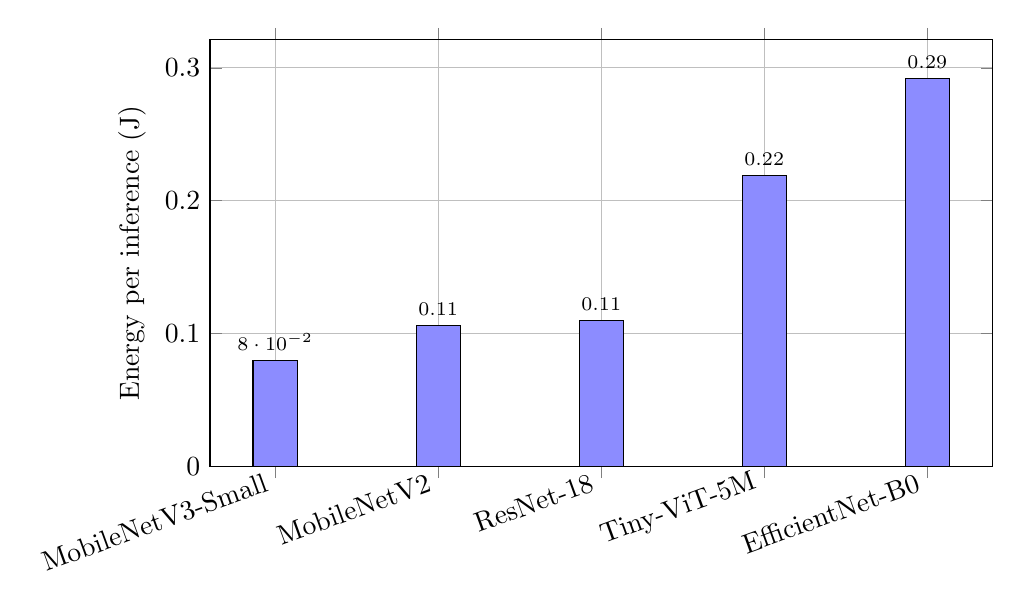
\begin{tikzpicture}
\begin{axis}[
    ybar,
    bar width=16pt,
    width=0.95\linewidth,
    height=7cm,
    ylabel={Energy per inference (J)},
    symbolic x coords={MobileNetV3-Small,MobileNetV2,ResNet-18,Tiny-ViT-5M,EfficientNet-B0},
    xtick=data,
    x tick label style={rotate=20,anchor=east},
    ymin=0,
    nodes near coords,
    every node near coord/.append style={font=\scriptsize},
    grid=major,
]
\addplot[fill=blue!45] coordinates {
    (MobileNetV3-Small,0.080)
    (MobileNetV2,0.106)
    (ResNet-18,0.110)
    (Tiny-ViT-5M,0.219)
    (EfficientNet-B0,0.292)
};
\end{axis}
\end{tikzpicture}
\caption{Measured energy per inference on Apple Silicon.}
\label{fig:measured-energy}
\end{figure}

\subsection{Latency and Energy}
Latency and energy are strongly aligned in this five-model Apple-Silicon study.
The Pearson correlation between latency and energy in the paper-aligned
synthetic evaluation is $r=0.9741$, which is consistent with the measured
ranking and the observation that the slower models are also more energy
expensive in this specific CPU-only deployment setting.

\begin{figure}[ht]
\centering
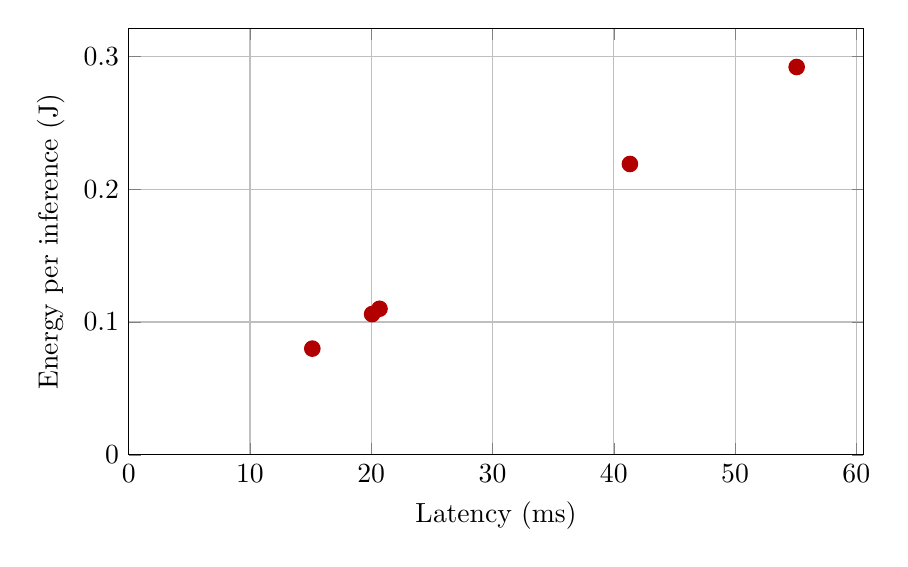
\begin{tikzpicture}
\begin{axis}[
    width=0.90\linewidth,
    height=7cm,
    xlabel={Latency (ms)},
    ylabel={Energy per inference (J)},
    ymin=0,
    xmin=0,
    grid=major,
]
\addplot[
    only marks,
    mark=*,
    mark size=2.8pt,
    color=red!70!black
] coordinates {
    (15.14,0.080)
    (20.07,0.106)
    (20.68,0.110)
    (41.33,0.219)
    (55.08,0.292)
};
\end{axis}
\end{tikzpicture}
\caption{Measured energy versus latency on Apple Silicon.}
\label{fig:energy-vs-latency}
\end{figure}

\subsection{Paper-Aligned Synthetic Fidelity}
The revised GAN was evaluated against the Apple-only grounded dataset derived
from the paper. Table~\ref{tab:fidelity} summarizes the fidelity metrics under
the corrected paper-aligned evaluation protocol. Direct distributional tests are
applied only to the modeled quantities, \texttt{energy\_J} and
\texttt{latency\_ms}. Power is evaluated as a derived quantity computed from
synthetic energy and latency, while repeated-trial energy spread is evaluated as
a per-model summary after variance calibration. Under this protocol, the model
matches energy, latency, and derived power well and preserves the measured
energy ranking perfectly.

\begin{table}[ht]
\centering
\caption{Fidelity of the paper-aligned GAN relative to the grounded Apple-only benchmark under the corrected paper-aligned evaluation protocol.}
\label{tab:fidelity}
\begin{tabular}{l c c c c}
\toprule
Feature & {Wasserstein} & {KS statistic} & {$p$-value} & Pass ($p>0.05$) \\
\midrule
Energy (\texttt{energy\_J}) & 0.003939 & 0.0636 & 0.1561 & Yes \\
Latency (\texttt{latency\_ms}) & 0.693447 & 0.0669 & 0.1195 & Yes \\
Derived power (\texttt{power\_W}) & 0.045739 & 0.0465 & 0.4984 & Yes \\
Repeated-trial energy spread (\texttt{energy\_std}) & 0.000000 & N/A & N/A & Matched \\
\bottomrule
\end{tabular}
\end{table}

\subsection{Measured versus Synthetic Means}
Table~\ref{tab:alignment} compares the paper's measured means against the means
of the paper-aligned synthetic dataset. Across all five models, the synthetic
means remain within approximately 1--4\% of the measured values.

\begin{table}[ht]
\centering
\caption{Measured versus paper-aligned synthetic mean metrics.}
\label{tab:alignment}
\begin{tabular}{l
S[table-format=1.3]
S[table-format=1.5]
S[table-format=2.2]
S[table-format=2.2]
S[table-format=2.2]
S[table-format=2.2]}
\toprule
Model &
{Measured $E$} &
{Synthetic $E$} &
{$E$ error (\%)} &
{Measured $L$} &
{Synthetic $L$} &
{$L$ error (\%)} \\
\midrule
MobileNetV3-Small & 0.080 & 0.08150 & 1.87 & 15.14 & 15.49 & 2.33 \\
MobileNetV2 & 0.106 & 0.10708 & 1.02 & 20.07 & 20.85 & 3.90 \\
ResNet-18 & 0.110 & 0.11169 & 1.54 & 20.68 & 20.97 & 1.39 \\
Tiny-ViT-5M & 0.219 & 0.22401 & 2.29 & 41.33 & 42.51 & 2.85 \\
EfficientNet-B0 & 0.292 & 0.29831 & 2.16 & 55.08 & 55.92 & 1.53 \\
\bottomrule
\end{tabular}

\vspace{0.4em}
\small
$E$ denotes energy in Joules and $L$ denotes latency in milliseconds.
\end{table}

\subsection{Supplemental Power and Synthetic Trial Spread}
Table~\ref{tab:supplemental} reports two model-specific quantities that were not
fully available in the original mean table: derived average power and synthetic
energy spread. The derived power values come directly from the paper's own
energy and latency values. The synthetic energy spread values come from the
paper-aligned GAN after within-model variance calibration and should be
interpreted as support estimates for repeated trials, not direct measurements.

\begin{table}[ht]
\centering
\caption{Supplemental power and synthetic repeated-trial spread estimates.}
\label{tab:supplemental}
\begin{tabular}{l
S[table-format=1.6]
S[table-format=1.6]
S[table-format=2.2]
S[table-format=1.6]}
\toprule
Model &
{Derived power (W)} &
{Synthetic power (W)} &
{Power error (\%)} &
{Synthetic energy std (J)} \\
\midrule
MobileNetV3-Small & 5.284016 & 5.297559 & 0.26 & 0.004455 \\
MobileNetV2 & 5.281515 & 5.167664 & -2.15 & 0.008113 \\
ResNet-18 & 5.319149 & 5.355765 & 0.69 & 0.007263 \\
Tiny-ViT-5M & 5.298814 & 5.305353 & 0.12 & 0.016725 \\
EfficientNet-B0 & 5.301380 & 5.375169 & 1.39 & 0.020086 \\
\bottomrule
\end{tabular}
\end{table}

\begin{figure}[ht]
\centering
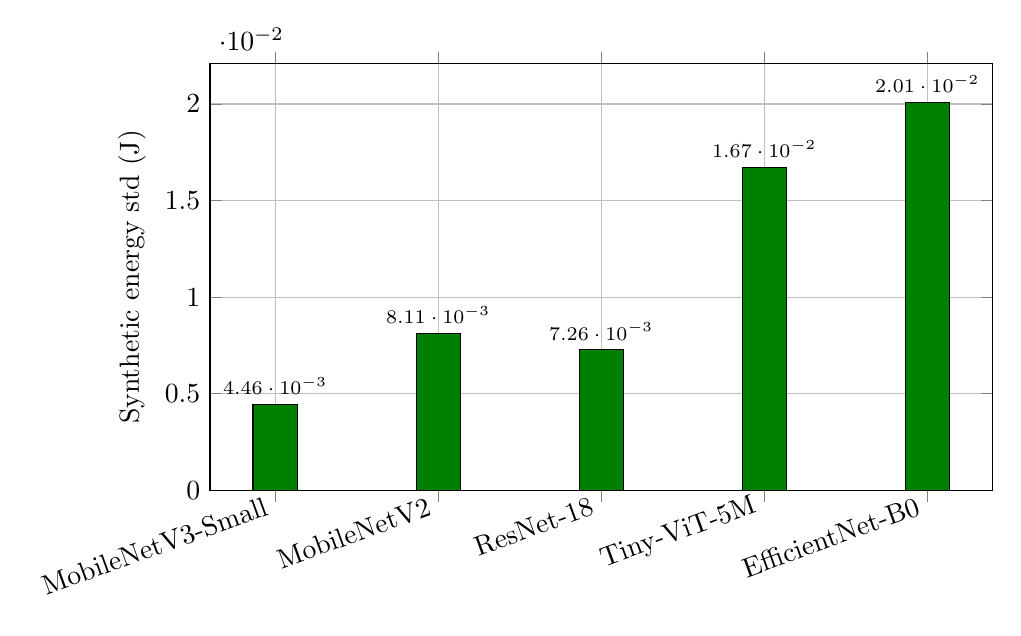
\begin{tikzpicture}
\begin{axis}[
    ybar,
    bar width=16pt,
    width=0.95\linewidth,
    height=7cm,
    ylabel={Synthetic energy std (J)},
    symbolic x coords={MobileNetV3-Small,MobileNetV2,ResNet-18,Tiny-ViT-5M,EfficientNet-B0},
    xtick=data,
    x tick label style={rotate=20,anchor=east},
    ymin=0,
    nodes near coords,
    every node near coord/.append style={font=\scriptsize},
    grid=major,
]
\addplot[fill=green!50!black] coordinates {
    (MobileNetV3-Small,0.004455)
    (MobileNetV2,0.008113)
    (ResNet-18,0.007263)
    (Tiny-ViT-5M,0.016725)
    (EfficientNet-B0,0.020086)
};
\end{axis}
\end{tikzpicture}
\caption{Synthetic repeated-trial energy spread by model for the calibrated paper-aligned Apple-Silicon dataset.}
\label{fig:energy-std}
\end{figure}

\section{Discussion}
The strongest version of this paper is the single-device version. Once the scope
is restricted to Apple Silicon, the claims become clear and defensible: the
benchmark identifies the most and least energy-efficient architectures in this
measured CPU-only setting, and it shows that common architectural proxies do
not fully explain the observed ordering.

The expanded 17-architecture sweep supports the same caution from a different
angle. It shows that parameter count, MACs, and FLOPs provide useful baselines,
but they still do not fully determine measured latency. For example, several
low-MAC depthwise or inverted-residual variants are slower than denser CNN or
mixer variants on this CPU-only PyTorch stack. Because the expanded sweep is
latency-only, it should be used as a reliability and baseline-comparison
artifact rather than as direct energy evidence.

Within that narrower scope, the synthetic component becomes easier to justify.
The revised GAN preserves the measured model ranking and reproduces mean energy
and latency closely, which makes it useful for supplemental repeated-trial
analysis and visualization. The synthetic support values are still secondary to
the measured benchmark, but they are now matched tightly to the exact device and
runtime configuration described in the paper.

The main remaining limitation is not the GAN itself but the granularity of the
original benchmark record. The paper does not publish measured trial-level
standard deviations or high-resolution per-model power traces. Consequently,
synthetic \texttt{energy\_std} and refined model-specific power should still be
described explicitly as derived or synthetic support quantities rather than as
direct measurements.

\section{Limitations and Future Work}
The central limitation of this paper is also its main strength: it remains a
single-device study. That narrow scope improves internal consistency, but it
also means the conclusions should be read specifically as claims about Apple
Silicon under CPU-only PyTorch inference, not as universal statements about edge
hardware more broadly.

That broader extension is now more concrete than it was in the earlier project.
A separate weaker-engine latency-only GAN workflow has already been built for
better-grounded non-Apple targets including Coral USB Accelerator, Coral Dev
Board, Raspberry Pi 4 CPU, and Snapdragon 888 NNAPI. Under its own evaluation
protocol, that weaker-engine model achieved a passing result with global
KS~=~0.0147, $p$~=~0.9997, full baseline coverage, a 100\% per-combination pass
rate, and mean per-combination latency error of about 0.26\%. Those results are
promising, but they belong in a separate comparative paper because they model
latency only and depend on heterogeneous public benchmark sources rather than
the tightly controlled Apple-Silicon benchmark used here.

Three directions would strengthen this Apple-Silicon study further:
\begin{enumerate}
\item publish measured standard deviations for energy directly from repeated
Apple-Silicon \texttt{powermetrics} runs matching the expanded 17-architecture
latency protocol;
\item save higher-resolution power traces per model so model-specific power
distributions can be analyzed directly rather than derived; and
\item extend the same benchmarking philosophy into a separate weaker-engine paper
that reports the already-developed non-Apple latency GAN results while adding
more directly measured baselines and harmonized runtime constraints.
\end{enumerate}

\section{Conclusion}
This Apple-Silicon-only manuscript shows that energy efficiency cannot be
reduced to FLOPs or parameter count alone even in a tightly controlled
single-device setting. Under CPU-only PyTorch inference on Apple Silicon,
MobileNetV3-Small is the most energy-efficient model in the tested set, while
EfficientNet-B0 is the least energy-efficient. Latency and energy are strongly
aligned, but theoretical complexity by itself is not enough to explain the full
ordering.

The supplemental synthetic component does not replace the benchmark. Its role is
to extend the Apple-Silicon measurement study with repeated-trial support data
that remain anchored to the measured means. That makes the paper stronger when
it is framed narrowly: as an Apple-Silicon inference-energy study with
supplemental synthetic trial modeling, rather than as a broad cross-device
hardware paper.

\begin{thebibliography}{16}

\bibitem{horowitz2014}
M.~Horowitz, ``Computing's energy problem (and what we can do about it),''
\emph{IEEE Micro}, vol.~34, no.~5, pp.~10--14, 2014.

\bibitem{mobilenet2017}
A.~G. Howard et al., ``MobileNets: Efficient convolutional neural networks for
mobile vision applications,'' \emph{arXiv preprint arXiv:1704.04861}, 2017.

\bibitem{mobilenetv22018}
M.~Sandler, A.~Howard, M.~Zhu, A.~Zhmoginov, and L.-C. Chen,
``MobileNetV2: Inverted residuals and linear bottlenecks,'' in
\emph{Proceedings of the IEEE Conference on Computer Vision and Pattern Recognition}, 2018.

\bibitem{mobilenetv32019}
A.~Howard, M.~Sandler, G.~Chu, et al., ``Searching for MobileNetV3,'' in
\emph{Proceedings of the IEEE International Conference on Computer Vision}, 2019.

\bibitem{efficientnet2019}
M.~Tan and Q.~Le, ``EfficientNet: Rethinking model scaling for convolutional
neural networks,'' in \emph{Proceedings of the International Conference on
Machine Learning}, 2019.

\bibitem{mittal2019}
S.~Mittal, ``A survey of techniques for improving energy efficiency of deep
learning,'' \emph{ACM Computing Surveys}, vol.~51, no.~2, 2019.

\bibitem{hardwareaware2019}
Y.~He et al., ``Understanding FLOPs is not enough: A study of hardware-aware
neural networks,'' \emph{arXiv preprint arXiv:1912.01090}, 2019.

\bibitem{eyeriss2017}
Y.-H. Chen et al., ``Eyeriss: An energy-efficient reconfigurable accelerator
for deep convolutional neural networks,'' \emph{IEEE Journal of Solid-State
Circuits}, 2017.

\end{thebibliography}

\end{document}
